\documentclass[letterpaper]{article}
\usepackage{underscore}
\usepackage[left=3.0cm, right=3.0cm, top=3.0cm]{geometry}
\usepackage[utf8]{inputenc}
\usepackage{graphicx}
\usepackage{graphics}
\usepackage[spanish]{babel}
\usepackage{lipsum}
\usepackage{float}
\usepackage{subfigure}
\usepackage{biblatex}
\usepackage{csquotes}
\usepackage{color}

\title{Circuitos de control de voltaje y corriente con tiristores}
\author{Carrasco Quiñones Karla Daniela y Reyna Gurrola Marcela}
\date{04 de Noviembre del 2019}

\begin{document}

\maketitle
\begin{center}
    
\includegraphics[scale=1.5]{Imagenes/Logo.png}\\
    \vspace{1cm}
Sistemas Electrónicos de Interfaz\\
Ing. Mecatrónica\\
4to. A
\end{center}
\newpage

\section{Objetivo}
Controlar voltaje y corriente alterna con un triac y un diac.

\section{Materiales}
\begin{itemize}
    \item Computadora con Orcad o Kicad
    \item 1 Potenciómetro de 100K o mayor
    \item 1 Capacitor cerámico de 0.33uF
    \item 1 diac
    \item 1 triac 
    \item 1 Foco
    \item Cable con clavija
    \item 1 Resistencia de 5.6k
    \item 1 Socket con cable
    \item Caimanes
    \item Protoboard
    \item Multímetro
\end{itemize}

\section{Procedimiento}
\begin{enumerate}
    \item Primero haz el circuito mostrado en la figura 1, el cual al ser simulado se comporta como lo haría un tiristor. Ten en cuenta que la terminal de la izquierda es la "gate" y las terminales de la derecha son las de las entradas 1 y 2 correspondientes.
    \item A continuación, realiza las simulaciones de 6 circuitos que utilizan el triac a modo de rectificador AC-DC, sin filtros. Estas son desde la figura 2 a la 13. Ten en cuenta que en el lugar de cada tiristor debes colocar el primer circuito mostrado en la figura 1. A excepción de los dos últimos circuitos, en los cuales debes usar un tiristor 1N1595, ya que al usar demasiados componentes Orcad no permite guardarlo y mucho menos mostrar cómo se comporta.
    \item Después simúlalos y observa como se llevan a cabo y actúan los voltajes y corrientes de las distintas configuraciones.
    \item Luego arma en la protoboard el circuito que se muestra en la figura 14. 
    \item Por último, haz marcas en el potenciómetro cuando la luz se encuentra apagada, cuando esta al mínimo brillo, cuando tiene un brillo medio y cuando se encuentra en su máximo brillo. Al medirlos valores del potenciómetro con ayuda del multímetro se pueden obtener el valor resistivo que genera las 4 distintas luminosidades del foco.
    
\end{enumerate}

\newpage

\section{Resultados}
El circuito para remplazar el triac para poderlo simular se muestra a continuación en la figura 1.
\begin{figure}[h]
    \centering
    \includegraphics[scale=0.35]{Imagenes/Tiristor.png}
    \caption{Circuito remplazo del triac.}
    \label{fig:my_label}
\end{figure}

El primer circuito a simular se muestra en la figura 2 es la configuración más básica en la que se puede usar el triac como rectificador.Debajo de este se encuentra su simulación correspondiente.
\begin{figure}[ht]
    \centering
    \includegraphics[scale=0.35]{Imagenes/Esquematico1.png}
    \caption{Rectificador controlado básico.}
    \label{fig:my_label0}
\end{figure}
\begin{figure}[ht]
    \centering
    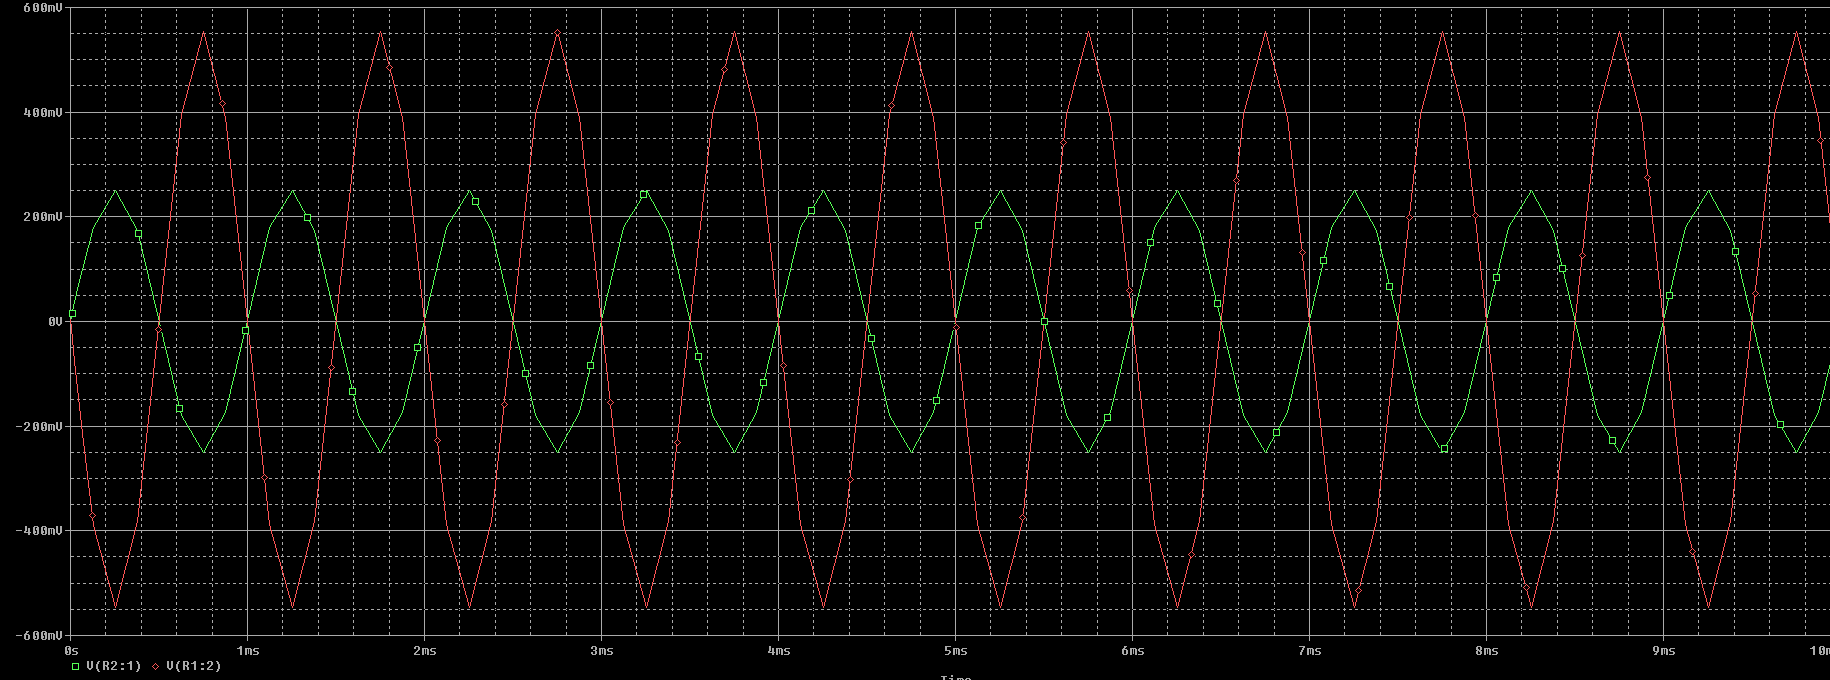
\includegraphics[scale=0.3]{Imagenes/Simulacion1.png}
    \caption{Tensión y corriente de salida del circuito 1.}
    \label{fig:my_label1}
\end{figure}

\newpage
El circuito número dos tiene una configuración en puente, se muestra en la figura 4 y su simulación en la figura 5.
\begin{figure}[ht]
    \centering
    \includegraphics[scale=0.5]{Imagenes/Esquematico2.png}
    \caption{Rectificador monofásico controlado.}
    \label{fig:my_label2}
\end{figure}
\begin{figure}[ht]
    \centering
    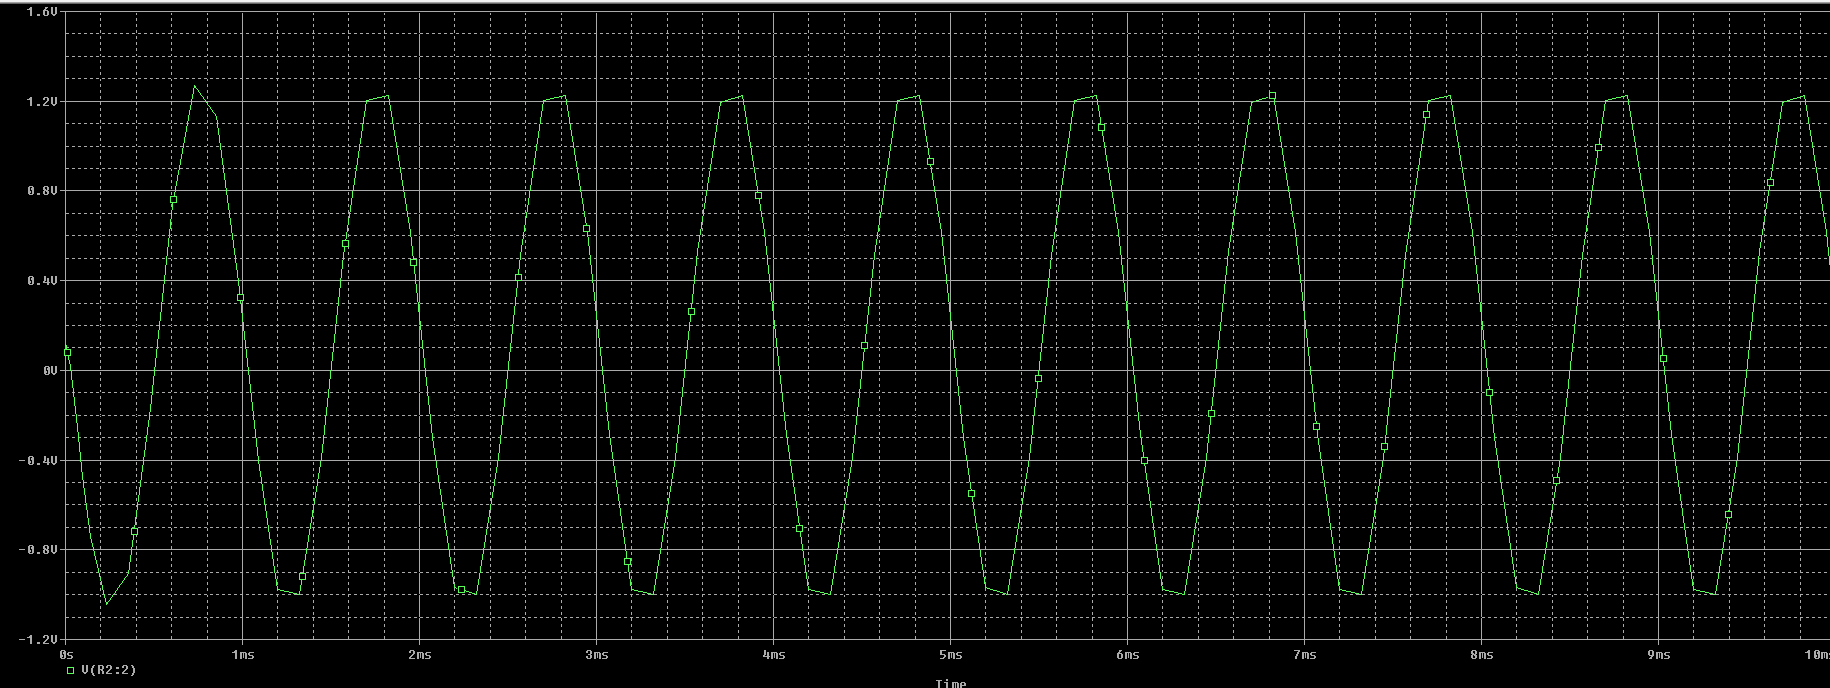
\includegraphics[scale=0.35]{Imagenes/Simulacion2.png}
    \caption{Voltaje de salida del circuito 2.}
    \label{fig:my_label3}
\end{figure}

\newpage
El circuito 3 (figura 6) es similar al anterior, solo que en este se agrega una carga a la salida. Por lo que el voltaje a la salida tendrá un valor fijo en el momento en que la intensidad de salida sea cero. Esto se puede observar en la figura 7.
\begin{figure}[ht]
    \centering
    \includegraphics[scale=0.5]{Imagenes/Esquematico3.png}
    \caption{Rectificador controlado con carga.}
    \label{fig:my_label4}
\end{figure}
\begin{figure}[ht]
    \centering
    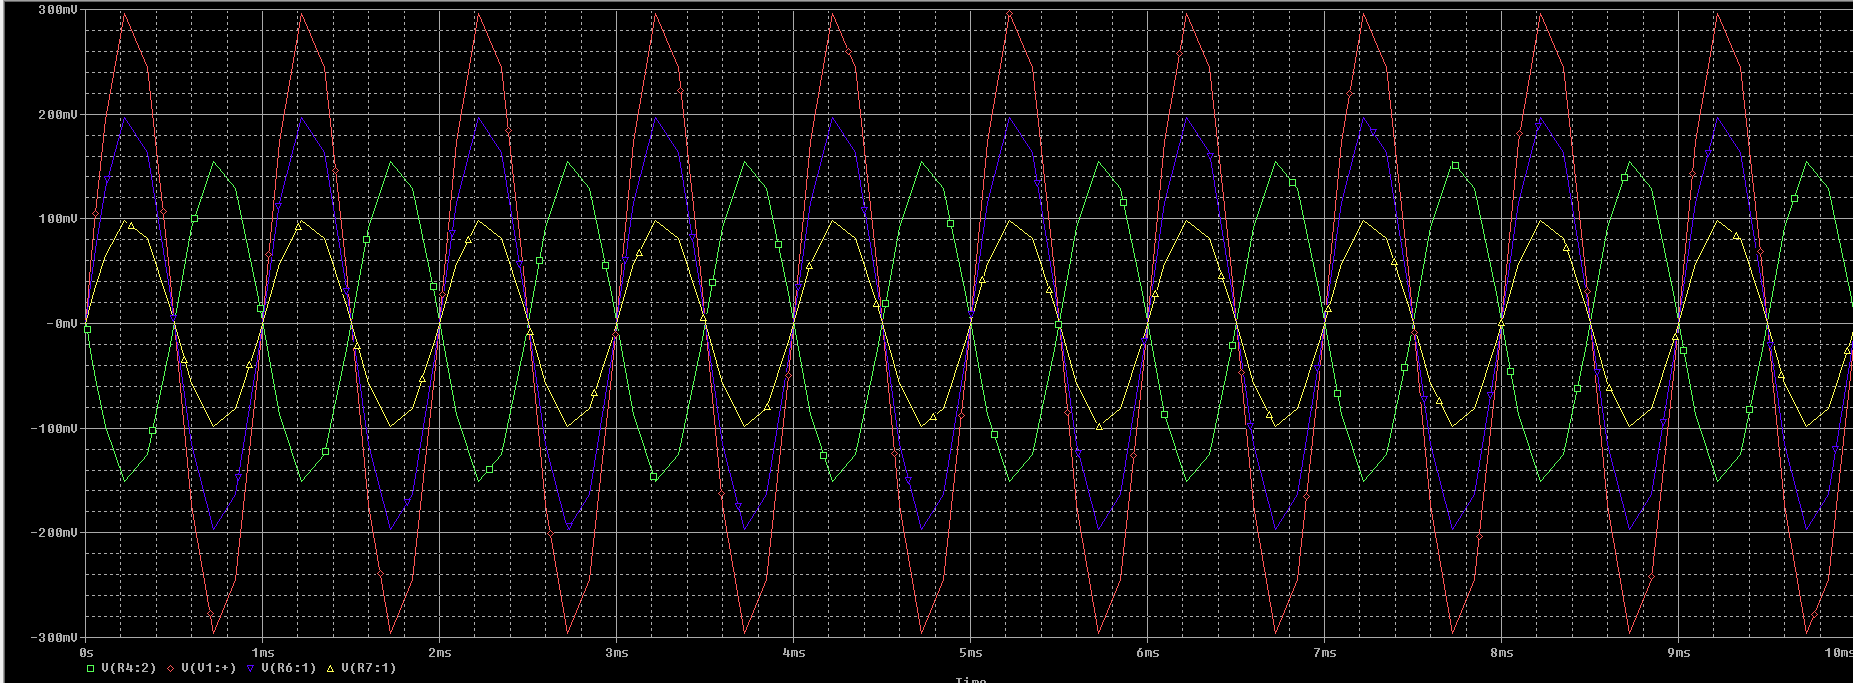
\includegraphics[scale=0.35]{Imagenes/Simulacion3.png}
    \caption{Voltaje de salida y corriente de entrada del circuito 3.}
    \label{fig:my_label5}
\end{figure}

\newpage
En el circuito 4, que se muestra en la figura 8, se utilizan dos triacs y dos diodos en puente. La simulación se muestra en la figura 9.
\begin{figure}[ht]
    \centering
    \includegraphics[scale=0.5]{Imagenes/Esquematico4.png}
    \caption{Rectificador semicontrolado.}
    \label{fig:my_label6}
\end{figure}
\begin{figure}[ht]
    \centering
    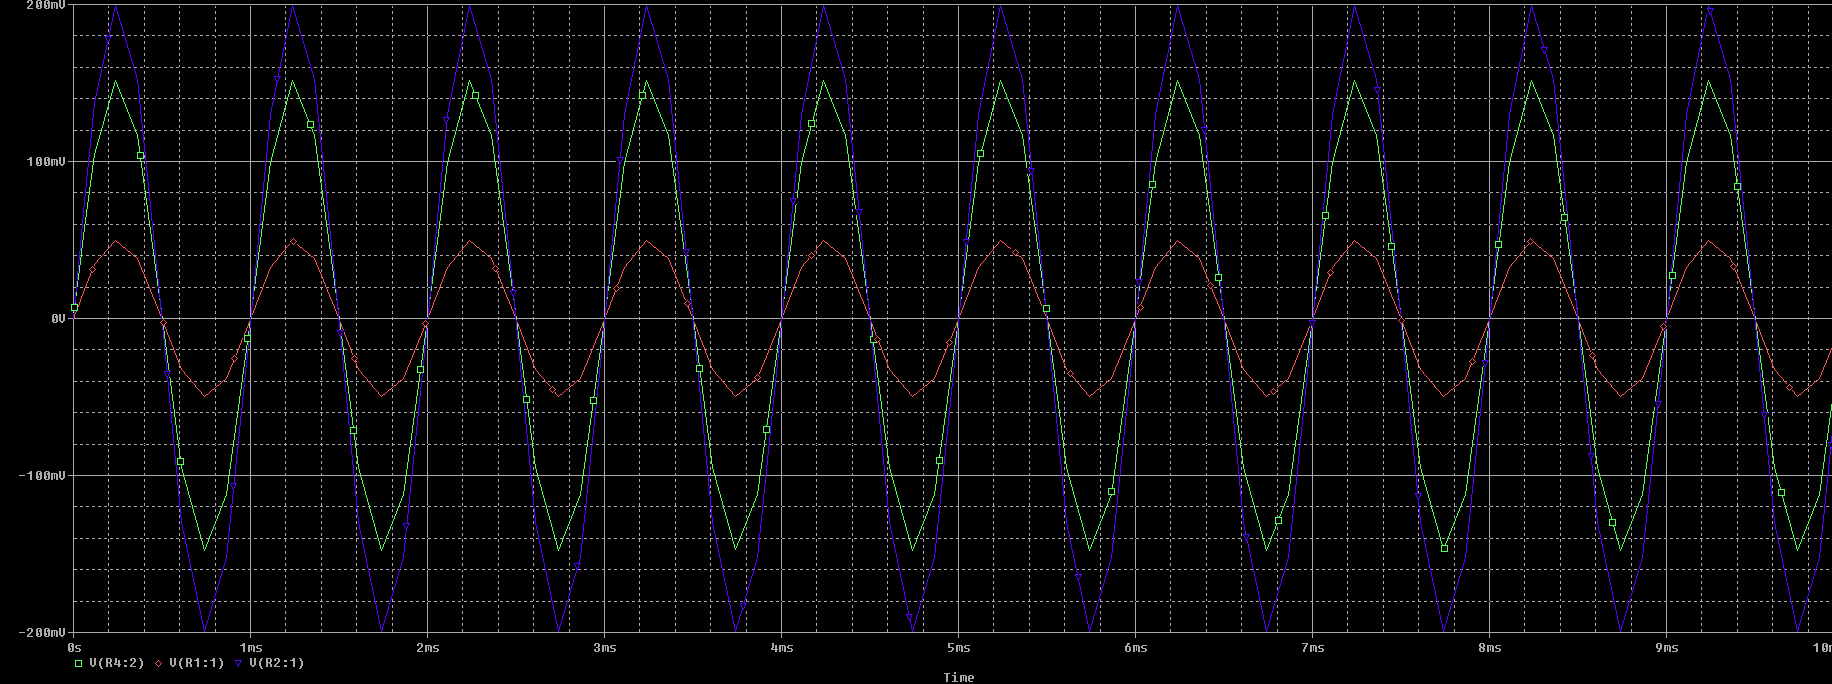
\includegraphics[scale=0.35]{Imagenes/Simulacion4.png}
    \caption{Voltaje de salida del circuito 4.}
    \label{fig:my_label7}
\end{figure}

\newpage
En el circuito 5 se trata de una conexión trifasica controlada, la cual se muestra en la figura 10, y su simulación se muestra en la figura 11.
\begin{figure}[ht]
    \centering
    \includegraphics[scale=0.6]{Imagenes/Esquematico5.png}
    \caption{Rectificador controlado trifásico con carga ideal.}
    \label{fig:my_label8}
\end{figure}
\begin{figure}[ht]
    \centering
    \includegraphics[scale=0.3]{Imagenes/Simulacion5.png}
    \caption{Voltaje de salida del circuito 5.}
    \label{fig:my_label9}
\end{figure}

\newpage
En el último circuito, figura 12, se tiene un resctificador trifásico semicontrolado, cuya simulación se muestra en la figura 13..

\begin{figure}[ht]
    \centering
    \includegraphics[scale=0.55]{Imagenes/Esquematico6.png}
    \caption{Rectificador trifásico semicontrolado.}
    \label{fig:my_labe20}
\end{figure}
\begin{figure}[ht]
    \centering
    \includegraphics[scale=0.3]{Imagenes/Simulacion6.png}
    \caption{Voltaje de salida del circuito 6.}
    \label{fig:my_labe21}
\end{figure}

\newpage
Ya para terminar se muestra el esquemático del circuito de control de voltaje y corriente con el tiristor en la figura 14 y respectivo PLC en la figura 15. Se agrego un block para conectar las entradas de voltaje como se muestran en el mismo diagrama.
\begin{figure}[ht]
    \centering
    \includegraphics[scale=0.5]{Imagenes/EsquematicoFoco.png}
    \caption{Esquemático armado.}
    \label{fig:my_labe22}
\end{figure}
\begin{figure}[ht]
    \centering
    \includegraphics[scale=0.5]{Imagenes/PLCFoco.png}
    \caption{PLC del circuito armado.}
    \label{fig:my_labe23}
\end{figure}

\section{Conclusión}
Carrasco Quiñones Karla Daniela:
\\Los transisitores de corriente solo conducen en un solo sentido, a causa de esto pudimos demostrar en la practica que estos permiten hacer una rectificación, esto mismo hacen los diodos pero estos podemos variar su tiempo y controlarlo al mismo tiempo y como se nos adecue a nuestras necesidades dependiendo de lo que querramos presentar en un tiempo futuro.\\
Los "Tiacs" y "Diacs" en este circuito permite el acceso de la corriente en ambos sentidos permitendo contolar la corriente alterna que es lo que necesitamos para susplantar el foco, ya que este es el funcionamiento del foco en este circuito.

Reyna Gurrola Marcela: 
\\Como lo demuestra la práctica, los tiristores permiten rectificar corriente alterna ya que estos solo conducen en un sentido, al igual que lo hacen los diodos, con la excepción de que a estos se les puede controlar al variar el tiempo de activación que se le aplica en el disparador. Mientras que el Diac y el Triac permiten el paso de la corriente en ambos sentidos, lo que los hace muy útiles al momento de controlar corriente alterna, que es lo que ocurre con el circuito del foco.'\\
Además cabe mencionar que se puede usar un Triac y un Diac para rectificar corriente alterna, con la diferencia de que cada semiciclo tendrá un valor positivo y negativo de manera intermitente.\\
Por último se sugiere que se utilice un potenciómetro de mayor valor en el circuito armado, ya que así se puede tener un mayor control sobre la intensidad del foco.


\end{document}
